\documentclass[11pt,a4paper,oneside]{report}

\usepackage{amsmath}
\usepackage{amssymb}
\usepackage{amsthm}
%\usepackage{array}
\usepackage{bbold}
%\usepackage{bm}
\usepackage[hypcap,small,hang]{caption}
%\usepackage{cite}
\usepackage{color}
\usepackage{dsfont}
%\usepackage{esint}
\usepackage{geometry}
\usepackage{graphicx}
\usepackage{wrapfig}
%\usepackage{hyperref}
%\usepackage{inputenc}
\usepackage{latexsym}
%\usepackage{listings}
\usepackage{mathrsfs}
\usepackage{mathtools}
\usepackage{microtype}
%\usepackage{marvosym}
%\usepackage{pdfpages}
%\usepackage{rotating}
%\usepackage{setspace}
\usepackage{slashed}
%\usepackage{times}
\usepackage{tikz}
%\usepackage{upgreek}
%\usepackage{url}
%\usepackage{wrapfig}
%\usepackage{showframe}
\usepackage[utf8]{inputenc}
\usepackage[T1]{fontenc}
\usepackage[pdftex,
            pdfauthor={Benny van Zuiden},
            pdftitle={libmd-intro},
            pdfsubject={An introduction to libmd},
            pdfkeywords={Theoretical Physics, Computational physics},
            pdfproducer={LaTeX},
            pdfcreator={Human},
            pdfborderstyle={/S/U/W 0}]{hyperref}
\usepackage{xmpincl}
 \includexmp{meta}
\usepackage{cleveref}

% New definition of square root:
% it renames \sqrt as \oldsqrt
\let\oldsqrt\sqrt
% it defines the new \sqrt in terms of the old one
\def\sqrt{\mathpalette\DHLhksqrt}
\def\DHLhksqrt#1#2{%
\setbox0=\hbox{$#1\oldsqrt{#2\,}$}\dimen0=\ht0
\advance\dimen0-0.2\ht0
\setbox2=\hbox{\vrule height\ht0 depth -\dimen0}%
{\box0\lower0.4pt\box2}}

\renewcommand{\theequation}{\arabic{section}.\arabic{equation}}
\renewcommand{\thesection}{\arabic{section}.}
\renewcommand{\thesubsection}{\alph{subsection}.}
\newcommand{\subsect}[1]{\subsection{#1} \setcounter{equation}{0}} 
\newcommand{\sect}[1]{\section{#1}  \setcounter{equation}{0}}

\renewcommand{\d}{\mathrm{d}}
\newcommand{\im}{\dot{\imath}}
\newcommand{\cs}[3]{\Gamma^{#3}_{#1 #2}}

%% TikZ related
\usetikzlibrary{calc}
\usetikzlibrary{shapes,arrows}
\tikzstyle{decision} = [diamond, draw, fill=blue!20,text width=4.5em, text badly centered, node distance=3cm, inner sep=0pt]
\tikzstyle{block} = [rectangle, draw, fill=yellow!20,text width=5em, text centered, rounded corners, minimum height=4em]
\tikzstyle{bblock} = [rectangle, draw, fill=red!20,text width=5em, text centered, rounded corners, minimum height=4em]
\tikzstyle{eblock} = [rectangle, draw, fill=green!20,text width=5em, text centered, rounded corners, minimum height=4em]
\tikzstyle{line} = [draw, -latex']
\tikzstyle{cloud} = [draw, ellipse,fill=red!20, node distance=3cm, minimum height=2em]

\begin{document}
\title{Algorithm Proposal}
\author{By Benny van Zuiden} 
%\date{\today}
%\maketitle
%\thispagestyle{empty}
%\newpage
%\tableofcontents
%\newpage

\begin{center}
{\textbf{\Large{\texttt{libmd}-intro}} \\*
\large{- By Benny van Zuiden -} \\*
{April - 8 - 2014} \\* {\vspace{4pt}}
\tiny{last revised April - 8 - 2014} \\* \vspace{10pt}}
\end{center}
\normalsize
\sect{Introduction to \texttt{libmd}}
\texttt{libmd} is a molecular dynamics library optimized for theoretical soft condensed matter physics. It is developed by:
\begin{center}
Benny van Zuiden\footnote{Maintainer.} (zuiden@ilorentz.org) \\
Jayson Paulose (paulose@ilorentz.org) \\
Thomas Beuman (beuman@ilorentz.org)
\end{center}
under the supervision of Vincenzo Vitelli. \texttt{libmd} is a object-oriented library written in \texttt{C++11} using nothing but the standard libraries and is tested to work on \texttt{gcc} and \texttt{LLVM/clang}. It uses \texttt{git} as a version control system, and \texttt{GNU make} as a build system. Parallel implementations for \texttt{cpu} is underway and implementations \texttt{gpu} planned. What makes \texttt{libmd} different from all the other molecular dynamics packages is that it is designed to solve typical soft matter problems, it designed to work in arbitrary dimensions and allows, is \emph{extremely} flexible, has multiple ways to make particles interact and constrain them and it can do dynamics in curved space (Monge patches).  
\sect{Introduction to molecular dynamics}
Molecular dynamics in the eyes of a theoretical softmatter physicist is nothing but the classical $N$-body problem --solved computationally. The classical $N$-body problem is basically solving Newton's equations of motion:
\begin{align}
a^{\mu}_i = \frac{1}{m_i} F^{\mu}_i
\end{align} 
Here $m_i$ is the mass of particle $i$, $a^{\mu}_i$ is the geodesic equations\footnote{In flat space: $a^{\mu}_i = \ddot{x}^{\mu}_i$, in curved space it's given by: $a^{\mu}_i = \ddot{x}^{\mu}_i+\cs{\rho}{\sigma}{\mu} \dot{x}^{\rho}_i \dot{x}^{\sigma}_i$.} and $F^{\mu}_i$ is probably non-trivial and based on lots of interactions. The classical $N$ body problem was analytically solved by Sundman and Wang and is of little practical use. Fortunately, it easy to solve the problem computationally --for most cases-- as time discretized. The error remains small if symplectic integrators --integrators that conserve Lagrangian symmetries are conserved -- are used. Typical integrators in flat space are symplectic Euler or velocity Verlet. For curves space we have developed our own.
\begin{figure}
	\begin{center}
    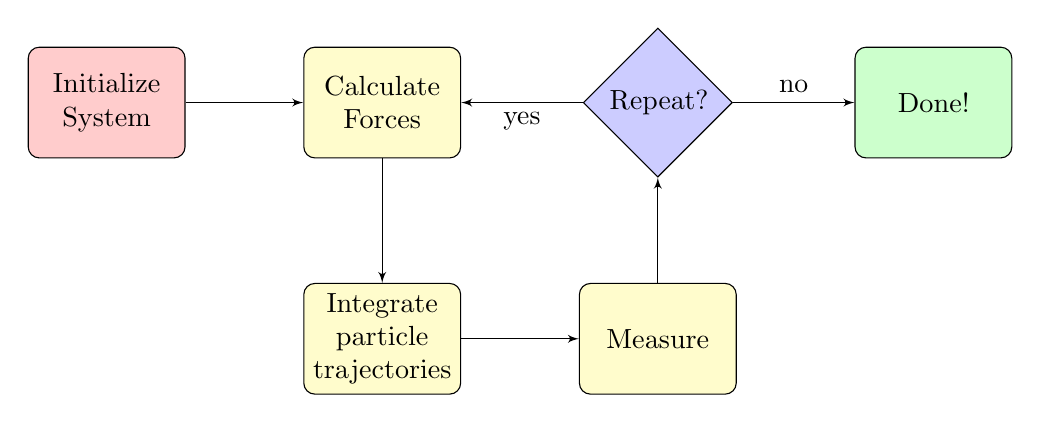
\begin{tikzpicture}[node distance = 2cm, auto]
    \node [bblock] (init) {Initialize System};
    \node [block, right of=init, node distance=3.5cm] (identify) {Calculate Forces};
    \node [block, below of=identify, node distance=3cm] (update) {Integrate particle trajectories};
    \node [block, right of=update, node distance=3.5cm] (evaluate) {Measure};
    \node [decision, above of=evaluate, node distance=3cm] (decide) {Repeat?};
    \node [eblock, right of=decide, node distance=3.5cm] (stop) {Done!};
    \path [line] (init) -- (identify);
    \path [line] (identify) -- (update);
    \path [line] (update) -- (evaluate);
    \path [line] (evaluate) -- (decide);
    \path [line] (decide) -- node {no}(stop);
    \path [line] (decide) -- node {yes}(identify);
  \end{tikzpicture}
  \end{center}
  \caption{A very basic schematic depicting how molecular dynamics is roughly done}
  \label{fig:md} 
\end{figure}
\\
As molecular dynamics is nothing less than an initial value problem, it requires initial conditions (possibly boundary conditions) and rules about how to calculate the forces. Once this is defined the integrator can calculate the particle trajectories sequentially using small time increments, called timesteps. After a bunch of timesteps one typically wants to measure a property after which the process can be repeated or terminated. This process is very schematically depicted in \cref{fig:md}.  
\sect{\texttt{libmd}-specific} 
\renewcommand{\theequation}{\arabic{section}.\alph{subsection}.\arabic{equation}}
In the following section we will explain how \texttt{libmd} is designed, what it can --and perhaps cannot-- do. Bear in mind that everything discussed in this is implemented regardless of dimensionality or presence of curvature --unless specifically stated otherwise.
\subsect{The simulation box}
\begin{wrapfigure}[15]{r}{0.4\textwidth}
    \begin{tikzpicture}[scale=0.5]
     \tikzstyle{every node}=[font=\tiny]
   	  \pgfmathsetmacro\lc{1.96188730425514123023821}
   	  \pgfmathsetmacro\r{0.866025403784438646763723}
   	  \pgfmathsetmacro\X{4.90471826063785307559552}
  	  \pgfmathsetmacro\Y{5.09713273454136756237537}
      \coordinate (Origin)   at (0,0);
      \coordinate (XAxisMin) at (-\X,0);
      \coordinate (XAxisMax) at (\X,0);
      \coordinate (YAxisMin) at (0,-\Y);
      \coordinate (YAxisMax) at (0,\Y);
      \coordinate (LL) at (-\X,-\Y);
      \coordinate (LR) at (\X,-\Y);
      \coordinate (TL) at (-\X,\Y);
      \coordinate (TR) at (\X,\Y);      
      \draw [thin, gray,-latex] (XAxisMin) -- (XAxisMax);
      \draw [thin, gray,-latex] (YAxisMin) -- (YAxisMax);
      \draw [thick,black] (LL) -- (TL) node[left,black,midway,font=\small] {$L^y$};
      \draw [thick,black] (LR) -- (TR);
      \draw [thick,black] (LL) -- (LR) node[below,black,midway,font=\small] {$L^x$};
      \draw [thick,black] (TL) -- (TR);
    \end{tikzpicture}
    \caption{A two dimensional box with dimensions $L^x$ by $L^y$. The origin of the box is where the grey axes cross.}
    \label{fig:box}
\end{wrapfigure}
We start by building a stage we the actors --particles-- can act. The stage is called the simulation box --simbox for short-- and has a hyper volume:
\begin{align}
V = \prod_\delta^D L^{\delta}
\end{align}
where $D$ is the dimension of the system and $L^{\delta}$ is the size of the box in each component. The origin $0^{\mu}$ is placed right in the middle of the box such that the boundaries of the box are present at every $\pm \tfrac{1}{2} L^{\delta}$. A two dimensional box is depicted in \cref{fig:box}. The boundaries can have boundary conditions per dimension. Currently, the implemented boundary are \texttt{NONE}, \texttt{PERIODIC} and \texttt{HARD} boundary conditions make perfectly bounce the particles. Additionally, the box can shrink, expand and shear.
\subsect{Particles}
Particles are the actor is in the box. Particles can be added and removed dynamically from the system. Additionally they can be pinned to one point. Every particle has the following properties:
\begin{itemize} \itemsep1pt \parskip0pt 
\item mass: $m$
\item position: $x^{\mu}$
\item velocity: $\dot{x}^{\mu}$
\end{itemize}
Additionally particles have:
\begin{itemize} \itemsep1pt \parskip0pt 
\item type\footnote{Types will be discussed in the next subsection.}
\item fix
\item forces acting on them: $F^{\mu}$
\end{itemize}
Internally they contain additional \emph{hidden} variables for better computational performance.
\subsect{Interactions} 
\emph{Without interactions life is boring}. Currently, the defined system is nothing but a box with a set of points, if we would calculate the equations of motion we would be simulating an ideal gas. To make it a bit more interesting --or realistic-- we have to define interactions. Interactions can be defined in many ways, for this part of the interaction implementation we will assume interactions are position depended and pairwise potentials. Mathematically:
\begin{align}
F^{\mu}_i=-\nabla \sum_{j>i} V(d(p_i,p_j))
\end{align}
Where $V$ is the pairwise potential and $d(p_i,p_j)$ is the distance between two particles. The potential $V$ can be any kind of potential Lennard--Jones or Yukawa for instance.
The Yukawa potential:
\begin{align}
V_Y(r)=\frac{b}{re^{\kappa r}}
\end{align}
Typical values for are $b=1$ and $\kappa=100$. Note that for these parameters $V(1) \approx 10^{-44}$  so it does not make sense to iterate over at large distances. Additionally making every particle interact with every other particle makes the algorithm at least order $N^2$ which is slow for a large number of particles. We can do better by creating some kind of cutoff radius $r_{co}$ and iterate over particles only within that cutoff vicinity, we can make the algorithm order $N log(N)$ which is typically better. In order to keep the potential continues we redefine the potential as:
\begin{align}
\tilde{V}_Y(r)=V_Y(r)-V_Y(r_{co})
\end{align}
The library can take any function $V: \mathds{R} \rightarrow \mathds{R}$ it generates the derivative automatically --without numerical errors and with the same complexity-- using a nice computational trick called \emph{automatic differentiation}.\\
Suppose you want certain particles to interact differently with other particles. A trivial way of doing this is by labeling particles with a type and then define interactions between types. Suppose I label a set of particles as type $0$ and the remaining particles as type $1$. I'll let $0$--$0$ interaction be Yukawa, $0$--$1$ interact Lennard--Jones and $1$--$1$ interact Yukawa with different parameters again. Or suppose you want to make a random spring network then you will need as many types as particles. If you don't like to think in types however, the code can translate bond lists to types for you.\\
Suppose you want to simulate dimers, trimers or polymers (or other weird objects for that matter). It can be done. We have included a structure in the code called superparticles that overrides type defined interactions if an interaction in the superparticle is assigned. This may sound a little vague so let me give an example. Take two particles of type $0$ and put them in the same superparticle, then within the super particle tie them together with a Hookean spring. The result is a dimer that interacts Yukawa with everybody else. Likewise you can create polymers and dimers. 
\subsect{External forces}
Additionally there is an external forces structure that allows you to add forces like linear gravity or damping, as well as any other kind of interaction you can write a function for. You can have multiple external forces acting on each particle. You can have damped interactions, multibody interactions, random kicking etc. The implementation of such forces is, however, a little harder.
\subsect{Curvature}
Adding curvature in the form of a Monge patch is near trivial. The Monge functions can be any (external) function $f: \mathds{R}^D \rightarrow \mathds{R} : C^2$ the code are automatically differentiates them.
\end{document}
